\documentclass[11pt]{article}
\usepackage{geometry}
\geometry{margin=1in}
\usepackage{graphicx}
\nonstopmode
\begin{document}

\begin{table}
\centering
\begin{tabular}{ll}
\hline
 citation             & wavelength range (nm)   \\
\hline
 \cite{Cooper_1995}   & 6.2 - 26.2              \\
 \cite{Wu_1985}       & 26.2 - 66.2             \\
 \cite{Metzger_1964}  & 66.2 - 76.2             \\
 \cite{Han_1989}      & 76.2 - 96.2             \\
 \cite{Walker_1955}   & 96.2 - 106.2            \\
 \cite{Nakayama_1964} & 106.2 - 116.2           \\
 \cite{Cheng_2011}    & 116.2 - 146.2           \\
 \cite{Smith_1991}    & 146.2 - 196.2           \\
 \cite{Wu_1989}       & 196.2 - 206.2           \\
 \cite{Chen_1991}     & 206.2 - 226.2           \\
 \cite{B_nilan_2000}  & 226.2 - 236.3           \\
\hline
\end{tabular}
\end{table}



\begin{figure}
\centering
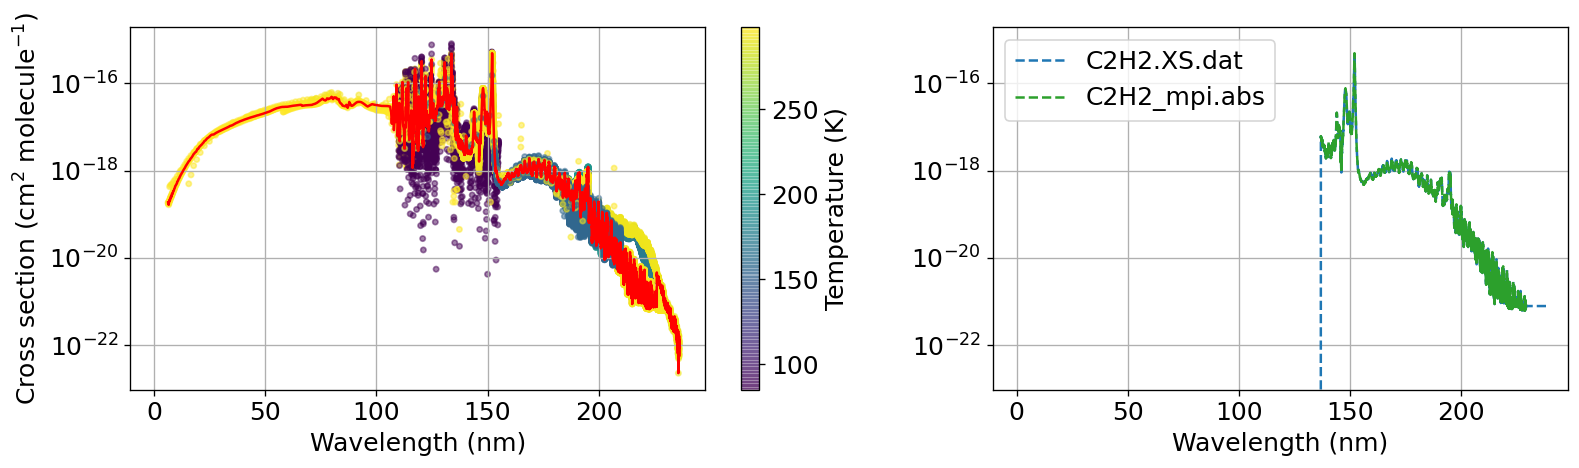
\includegraphics[width=\textwidth]{C2H2.png}
\caption{C2H2}
\label{fig:C2H2}
\end{figure}


\bibliographystyle{unsrt}
\bibliography{C2H2}
\end{document}